 \documentclass [12pt]{article} 

\usepackage {amsmath}
\usepackage {amsthm}
\usepackage {amssymb}
\usepackage {graphicx} 
\usepackage {float}
\usepackage {multirow}
\usepackage {xcolor}
\usepackage {algorithmic}
\usepackage [ruled,vlined,commentsnumbered,titlenotnumbered]{algorithm2e} \usepackage {array} 
\usepackage {booktabs} 
\usepackage {url} 
\usepackage {parskip} 
\usepackage [margin=1in]{geometry} 
\usepackage [T1]{fontenc} 
\usepackage {cmbright} 
\usepackage [many]{tcolorbox} 
\usepackage [colorlinks = true,
            linkcolor = blue,
            urlcolor  = blue,
            citecolor = blue,
            anchorcolor = blue]{hyperref} 
\usepackage {enumitem} 
\usepackage {xparse} 
\usepackage {verbatim}
\usepackage{listings}
\usepackage{xcolor}
\lstset { %
    language=C++,
    backgroundcolor=\color{black!5}, % set backgroundcolor
    basicstyle=\footnotesize,% basic font setting
}
\newtheorem{theorem}{Theorem}
\newtheorem{remark}{Remark}
\newtheorem{lemma}[theorem]{Lemma}
\theoremstyle{definition}
\newtheorem{definition}{Definition}[section]
\newtheorem{claim}{Claim}




\DeclareTColorBox {Solution}{}{breakable, title={Solution}} \DeclareTColorBox {Solution*}{}{breakable, title={Solution (provided)}} \DeclareTColorBox {Instruction}{}{boxrule=0pt, boxsep=0pt, left=0.5em, right=0.5em, top=0.5em, bottom=0.5em, arc=0pt, toprule=1pt, bottomrule=1pt} \DeclareDocumentCommand {\Expecting }{+m}{\textbf {[We are expecting:} #1\textbf {]}} \DeclareDocumentCommand {\Points }{m}{\textbf {(#1 pt.)}} 

\begin {document} 

\vspace {1em} 
\begin {Instruction} 
Adapted From Virginia Williams' lecture notes.
\end {Instruction}  

{\LARGE \textbf {COMP 285 (NC A\&T, Spr `22)}\hfill \textbf {Lecture 23} } 

\begin{centering}
\section*{Single-Source Shortest Paths with Negative Edge Weights}
\end{centering}

\section{Bellman-Ford Algorithm} 
In this section, we study the Bellman-Ford algorithm that solves the single source shortest paths problem on graphs with edges with potentially negative weights. Given a directed graph $G = (V, E)$ with edge weights given by $w(x, y )$ for $(x, y ) \in E$, we want to compute the shortest path distances $d(s, v )$ from source $s$ for all $v \in V$ . More specifically, the Bellman-Ford algorithm: 

\begin{itemize}
  \item Detects a negative cycle if it exists and is reachable from $s$, or 
  \item Computes the shortest path distances $d(s, v )$ for all $v \in V$
\end{itemize} 

Note $\pi(\cdot)$ is used to store the shortest paths found and $\pi(v )$ represents the predecessor of $v$ on the shortest path from $s$ to $v$.

\textbf{NOTE}: This version of Bellman-Ford is a bit different than the one we presented in class! As mentioned in class, we changed it up slightly to be more in line Dynamic Programming. However, the analysis is basically the same. We'll analyze the above version here.

\begin{algorithm}
\caption{Bellman-Ford Algorithm}
\label{alg:1}
\begin{algorithmic}
\STATE $d[v] \gets \infty, \forall v \in V$ \texttt{// set initial distance estimates}
\STATE \texttt{to maintain paths: set } $\pi(v) \gets $nill for all $v, \pi(v)$ represents the predecessor of $v$
\STATE $d[s] \gets 0$ \texttt{// set distance to start node trivially as 0}
\FOR{$i$ from $1 \to n - 1$}
  \FOR{$(u,v) \in E$}
    \STATE $d[v] \gets \min\{d[v], d[u] + w(u,v) \}$ \texttt{// update the distance estimates for v}
    \STATE \texttt{to maintain paths, if } $d[v]$ \texttt{changes, then } $\pi(v) \gets u$
  \ENDFOR
\ENDFOR
\STATE \texttt{// Negative Cycle Step}
\FOR{$(u,v) \in E$}
  \IF{$d[v] > d[u] + w(u,v)$}
    \RETURN "Negative Cycle" \texttt{// negative cycle detected}
  \ENDIF
\ENDFOR
\RETURN $d[v] \forall v \in V$
\end{algorithmic}
\end{algorithm}

For an example run of the Bellman-Ford algorithm, please refer to the lecture slides or CLRS.

The total runtime of the Bellman-Ford algorithm is $O(mn)$. In the first for loop, we repeatedly update the distance estimates $n - 1$ times on all $m$ edges in time $O(mn)$. In the second for loop, we go through all $m$ edges to check for negative cycles in time of $O(m)$. 

We prove the correctness of the Bellman-Ford algorithm in two steps:

\begin{claim}[If there is a negative cycle reachable from $s$, then the Bellman-Ford algorithm detects and reports ``Negative Cycles'']
\begin{proof}

For the sake of contradiction, suppose there exists a negative cycle $C$ reachable from the source $s$ and the Bellman-Ford algorithm does not report ``Negative Cycles''. Assume $C$ contains nodes $v_1, v_2, \cdots , v_k$ with edges $(vi , vi+1)$ for $i = 1, \cdots , k$ such that $\sum^{k}_{i=1} w(vi , vi+1) < 0$, where $v_k+1 = v_1$. See Figure \ref{fig:cycle}. Let $d[\cdot]$ be the distance estimates determined in the first for loop of the algorithm. Since $C$ is reachable from $s$, there is a path from $s$ to $v_1$ and to all nodes on $C$. In particular, there exist simple paths, i.e., paths without cycles, of at most $n - 1$ edges to the nodes of $C$. In the first for loop, the edges on each such simply path get relaxed in order and consequently, $d[vi ]$ will be some finite number less than $\infty$ for $i = 1, \cdots , k$. Since the Bellman-Ford algorithm does not report ``Negative Cycles'' in the second for loop, it must be that $d[vi+1] \leq d[vi ] + w(vi , vi+1)$ for $i = 1, \cdots , k$. Adding the inequalities, we obtain
$$
\sum_{i=1}^k d[v_{i+1}] \leq \sum_{i=1}^k d[v_i] + w(v_i, v_{i+1})
$$


\begin{figure}
\centering
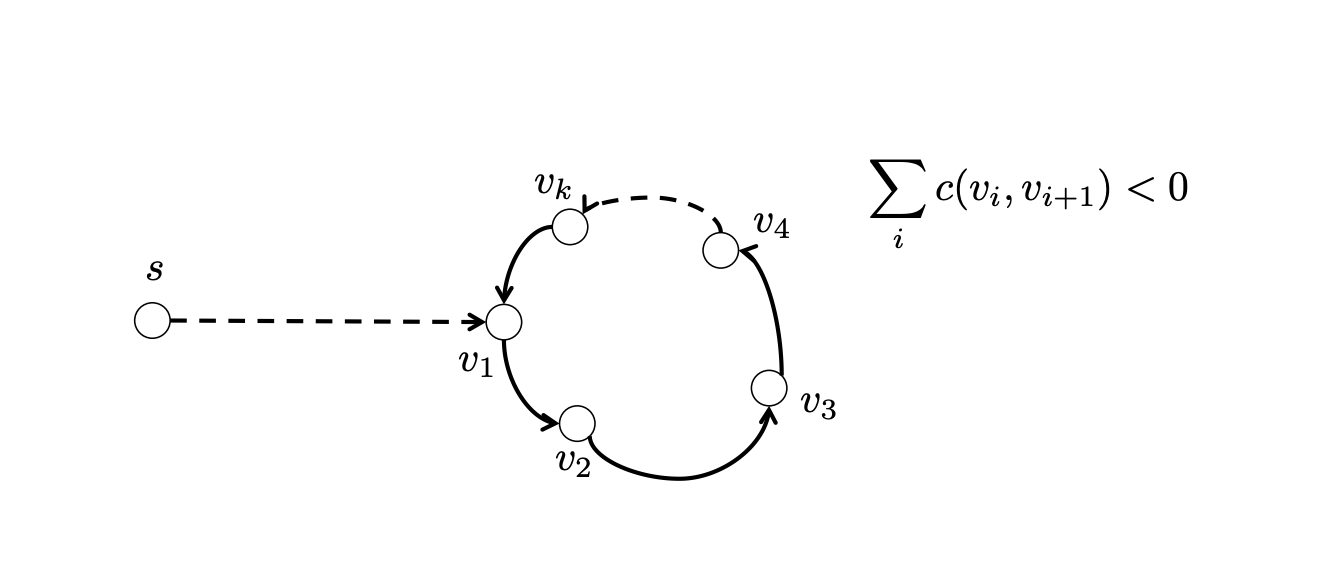
\includegraphics[scale=0.5]{Cycle.png}
\caption{A negative cycle reachable from source $s$}
\label{fig:cycle}
\end{figure}
 
As we are summing over the cycle $C$, the terms $\sum_{i=1}^k d[v_{i+1}]$ and $\sum_{i=1}^k d[v_i ]$ are equal and can be cancelled. It follows that $0 \leq \sum_{i=1}^k w(vi , vi+1)$. This contradicts that $C$ is a negative cycle.

\end{proof}
\end{claim}

In the next claim, we show that if the graph has no negative cycles reachable from the source, then the Bellman-Ford algorithm returns the correct shortest path distances. 

\begin{claim}[If G has no negative cycles reachable from $s$, then $d[v\text{]} = d(s, v ), \forall v \in V$]

\begin{proof} 

Let $d_k (v )$ be the value of $d[v ]$ after $k$ iterations of the first for loop. We prove by induction the statement that $d_k (v )$ is at most the minimum distance of a path from $s$ to $v$ with at most $k$ edges. Then, we will have $d_{n-1}(v ) = d[v ]$ for all node $v$ at termination. We'll argue below that if there is any path from $s$ to $v$ , then there is some shortest path with at most $n - 1$ edges, so this means 
$$
\text{dist}(s, v ) \leq d[v ] = d_{n-1}(v ) \leq \text{ minimum cost of a path with at most } n - 1 \text{ edges } = \text{dist}(s, v )
$$

Thus, everything in the above inequality chain is equal, and in particular $d[v ]$ is equal to the distance from $s$ to $v$ . Above, we used the fact that $d[v ]$ is an over-estimate on dist$(s, v )$, which follows from our analysis of Dijkstra's algorithm. 

We now argue that if there is a path from $s$ to $v$ , then there exists a shortest path from $s$ to $v$ has at most $n - 1$ edges. If a shortest path has a cycle, the cycle cannot be negative and we can remove it and improve its total distance. If the cycle has a positive weight, removing the cycle will strictly improve the shortest path's distance. If the cycle has zero weight, we can ignore the cycle. Hence, we can assume that shortest paths are simple, that is, do not have cycles. 

\textit{Base Case}: When $k = 0$, the distance estimates have been just initialized. So, $d_0(v ) = \infty$ if $v \neq s$. Furthermore, $d_0(s) = 0 = d(s, s)$, which is the minimum distance of length-$0$ paths from $s$ to $s$. The statement is satisfied for the base case. 

\textit{Inductive Step}: Assume that $d_{k-1}(v )$ is at most the minimum distance of a $s \to v$ path on at most $k - 1$ edges for all $v$. 

Consider $v \neq s$. Let $P$ be a shortest simple $s \to v$ path on at most $k$ edges. Let $u$ be the node just before $v$ on $P$, and let $Q$ be the sub-path of $P$ from $s$ to $u$. The path $Q$ would have at most $ k - 1 $ edges and is a shortest path from $s$ to $u$ with at most $k - 1$ edges, since sub-paths of shortest paths are also shortest paths. By the inductive hypothesis, $Q$ has cost at most $d_{k-1}(u)$. In the $k$-th iteration, we update $d_k (v )$ such that $d_k (v ) \leq d_{k-1}(u) + w(u, v ) \leq w(Q) + w(u, v ) = w(P)$. The induction is complete, and the claim is proved.

\end{proof}
\end{claim}

\section{Amortized Time}
Let's return to the Fibonacci heaps that we only very briefly mentioned above.
 
Note the runtimes listed for the operations of Fibonacci heaps are not worst-case runtimes. Instead, they are, what we call amortized runtimes. We say an operation on a data structure takes amortized $t(n)$ time if starting from an empty data structure, performing the operation
$L$ times takes $O(L \times t(n))$ time in total. This means the runtime of the operation is $O(t(n))$ when averaged over the sequence of $L$ instances of the operation. Each individual operation call may take much more than $t(n)$ time, but this is compensated by many cheap operation calls (that take much less than $t(n)$ time).
 
We analyze the amortized cost of incrementing a binary counter by one when the count is represented in binary. Consider a b-bit counter which starts at $0$ (i.e. b $0$'s). In each increment operation, we update the counter's bits correspondingly by flipping some bits from $0$ to $1$, or vice versa.

Some of the increment operations may take $\Omega(b)$ time. For example, an increment operation can require carrying $b$ bits:

\begin{align*}
1111111& \\
+ 1& \\
= 10000000&
\end{align*}

Other increments may take $O(1)$ time. 
\begin{align*}
10000000& \\
+ 1& \\
=10000001& \\
\end{align*}
 
All this said, we can show the amortized cost of the increment operation on a binary counter is $O(1)$. Even though some increments take time linear in the number of bits, if we do $n$ increment operations to the counter starting from the all $0$s, each operation takes $O(1)$ time on average.

\begin{claim}{The total time to increment a binary counter $n$ times is $O(n)$} 

We use what is known as the \textit{accounting} method to prove this claim. Each nonzero bit in the binary counter will get a ``credit'' obtained from earlier increment operations that will then be used to pay for later expensive operations. More specifically, we will maintain the invariant that every $1$ in the binary representation has a ``credit'', which we represent as $\bigoplus$, associated with it. Let $x$ be the binary counter. If we start with an ``empty'' integer – that is $0$ – then clearly all $1$'s have a ``credit'' as there are no $1$'s. Assume that all the 1's of $x$ have a ``credit'' at the start of an increment operation. In each increment operation, we know the first addition will require constant work for which the addition operation will be charged with. We actually ``charge'' the addition operation two ``credit''s, represented as $\bigoplus\bigoplus$, to the new $1$ to be added:

\begin{align*}
x = 1^{\bigoplus}1^{\bigoplus}0& \\
+& \\
1^{\bigoplus \bigoplus}
\end{align*}

Now we start adding. We will maintain the invariant that any ``carry'' bit will have two $\bigoplus$ credits. For completeness, we'll call the original $1$ to be added to $x$ a ``carry'' as well. 

Now, at each point we are adding a carry bit to a bit in $x$. If the carry bit is $0$, we do nothing and stop. If the carry bit to be added to the $i$-th bit is $1$ and the $i$-th bit of $x$ is $0$ (Note $i$ starts at $0$), then one of the $\bigoplus$ credits of the carry bit is used to store $1$ in $x[i]$ and the other remains on this new 1 as $\bigoplus$:

\begin{align*}
x = 1^{\bigoplus}1^{\bigoplus}0& \\
+ 1^{\bigoplus \bigoplus} \\
= 1^{\bigoplus}1^{\bigoplus}1^{\bigoplus} &
\end{align*}
At this point, the carry for the $i + 1$-st slot is $0$ and we can stop the addition.

When the carry bit to be added to the $i$-th bit is $1$ and $x[i]$ is $1$, however, we will get a non-zero carry bit for the $i + 1$-st position. In this case, we will use one $\bigoplus$from the $1$ stored in $x[i]$ to pay for storing a $0$ in $x[i]$ (doing the carry addition), and we'll move the two $\bigoplus$ of the carry bit to the new carry bit for the $i + 1$-st position. This maintains the invariant thatall $1$s in $x$ have a credit and all carries have two credits.

For example, consider an increment operation on the binary counter $x = 0111$:

\begin{align*}
01^{\bigoplus}1^{\bigoplus}1^{\bigoplus}& \\
+1^{\bigoplus\bigoplus}&
\end{align*}

A new carry bit is formed:
\begin{align*}
&1^{\bigoplus\bigoplus}\\
=01^{\bigoplus}&1^{\bigoplus}0 
\end{align*}

A new carry bit is formed:
\begin{align*}
&1^{\bigoplus\bigoplus}\\
=0&1^{\bigoplus}00 
\end{align*}

A new carry bit is formed:
\begin{align*}
&1^{\bigoplus\bigoplus}\\
=&0000 \\
=&1^{\bigoplus}000
\end{align*}
\end{claim}

All carry propagations of additions are for free because they are paid for by the credits accumulated in previous additions of $0$'s and $1$'s. There are $O(n)$ credits overall, two for each increment operation. Thus, the total runtime is $O(n)$. The credit system allows you to pay for later long operations by depositing credits from previous short operations. Some operations are long, but over all $n$ increment operations, the total work is $O(n)$. It follows that the increment operation takes amortized $O(1)$ time.

\end{document}